% !TeX root = ../SPL-Challenges.tex
% !TeX spellcheck = en_US

\section{Leaderboard Challenges}
Starting in 2025, several leaderboards will be introduced to track and compare team performances across key skills
over multiple years. These leaderboards aim to motivate teams to improve in specific areas deemed valuable by the
league and to compile a record of the top-performing components and skills. By highlighting these individual skills,
the league encourages focused development in areas that contribute to overall team performance, and creates a showcase
of the best technical abilities in the league.

\subsection{Challenge Rules}
Each year, teams can choose to make an attempt at specific leaderboard challenges. The Technical Committee and Organizing
Committee will coordinate dedicated time slots at RoboCup for teams to complete their leaderboard attempts.
Metrics from each attempt will be recorded and added to the appropriate leaderboard. Each leaderboard will be based
on unique metrics and procedures, detailed below. Teams must indicate their intention for a leaderboard attempt 2 weeks before
the first competition day.

\subsection{Fastest Walk Leaderboard}
This leaderboard will measure how fast a NAO will be able to navigate along a both a straight path and one with obstructions.

\subsubsection{Setup}
This leaderboard challenge will take place on one half of a standard SPL field, and requires 1 active robot and 4 inactive robots.
Inactive robots will act as obstacles for half of the attempt and will be placed as follows (illustrated in \cref{fig:walk_leaderboard}):
\begin{itemize}
    \item On the penalty mark
    \item On both corners of the goal area that are not touching the field boundary
    \item On the corner of the goal area closest to the competing robot
\end{itemize}

The competing robot will be placed on the touchline, in line with the penalty mark.
The end goal is the touchline on the other side of the field.

\begin{figure}[t]
    \centerline{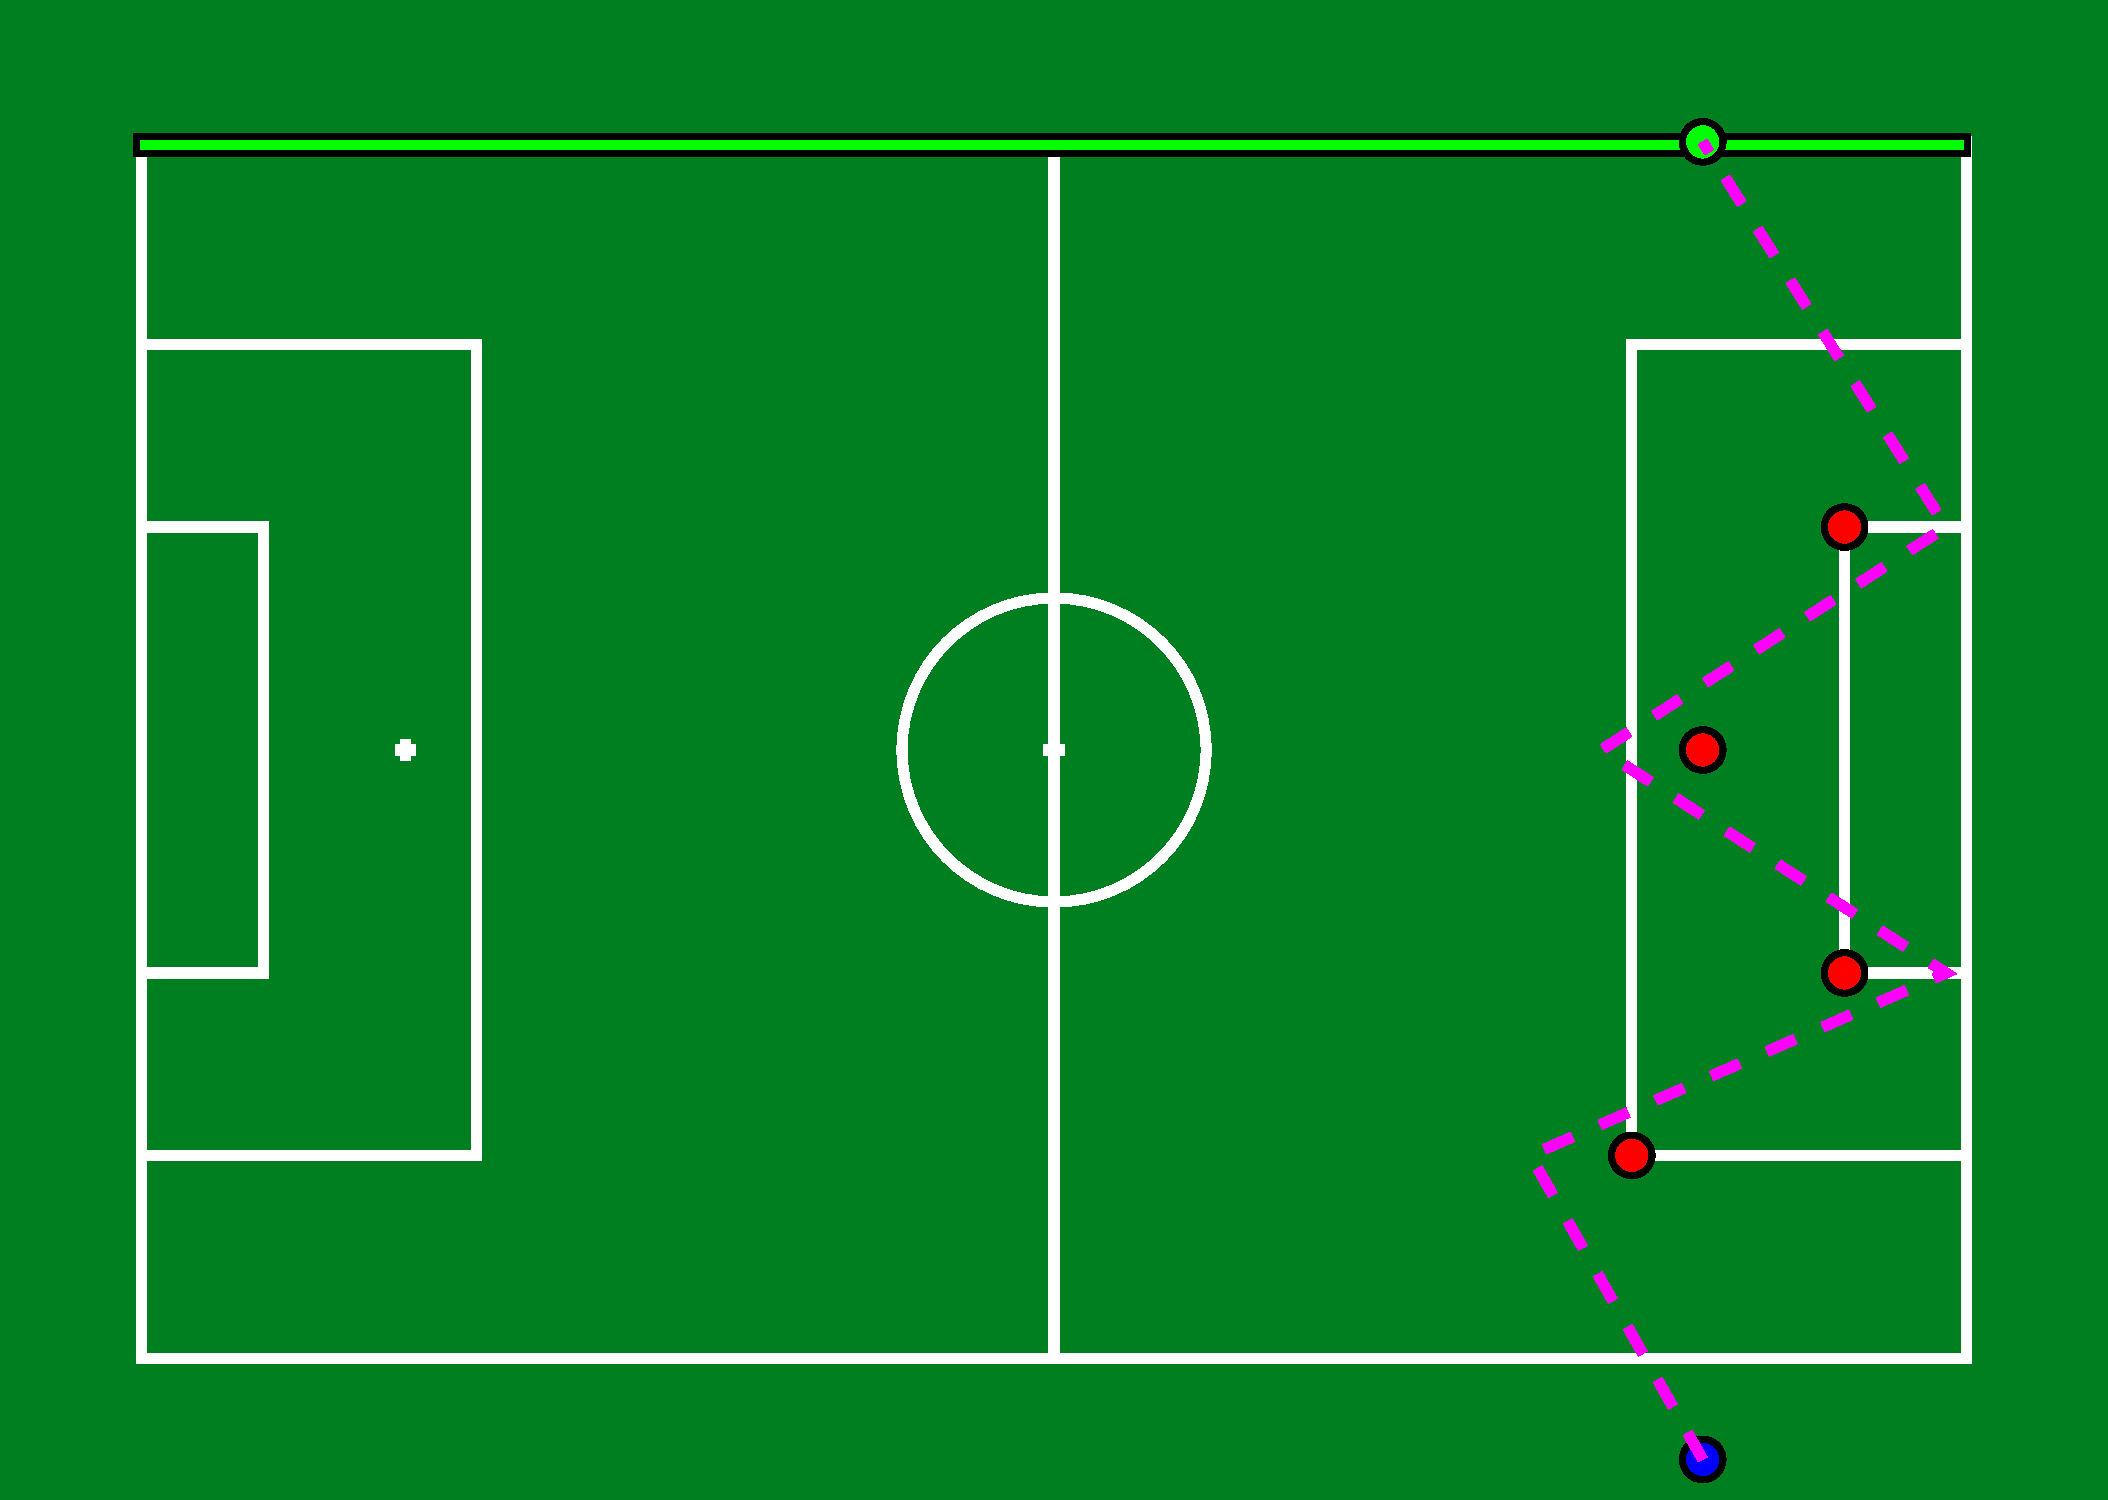
\includegraphics[width=\columnwidth]{figs/walk_leaderboard.pdf}}
    \caption{Fastest Walk Leaderboard: Robot completing the attempt is shown in blue, target is shown in green, obstacles are shown in red. An example path is shown in magenta}
    \label{fig:walk_leaderboard}
\end{figure}

\subsubsection{Challenge Execution}
Two types of runs will be completed, with three attempts per run allowed.

One run will be with the obstacles in place, where the active robot will need walk from it's
starting position to the target touchline, while weaving around the obstacle robots. (see \cref{fig:walk_leaderboard} for an example)

The other run will be with no obstacles, where the active robot will just need to walk 
to the target touchline.

Participating teams can choose which order they wish to complete these runs. Code changes are not allowed during a run,
but are allowed between runs.

Participating teams must start the robot behaviour of their competing robot via a single chest button
press (this mimics the chest button behaviour of switching between playing and penalized state).
The participating robot must navigate autonomously and cannot be remote controlled during the challenge

\subsubsection{Scoring}
Time starts from when the chest button is pressed, to when to robot entirely crosses the target touchline.

Teams will take 3 attempts at navigating both runs, with the sum of the lowest time for each
run being recorded in the leaderboard. Times will be rounded to the nearest second.

\subsection{Best Kick Leaderboard}
This leaderboard will measure how far and how accurate a NAO will be able to kick a standard
SPL soccer ball.

\subsubsection{Setup}
This leaderboard challenge will take place on a standard SPL field, and requires 1 active robot and 1 ball.
The ball will be placed on the centre of the edge of the goal area, in line with the penalty mark.
The competing robot will be placed in the centre of the goaline facing the ball
\begin{figure}[t]
    \centerline{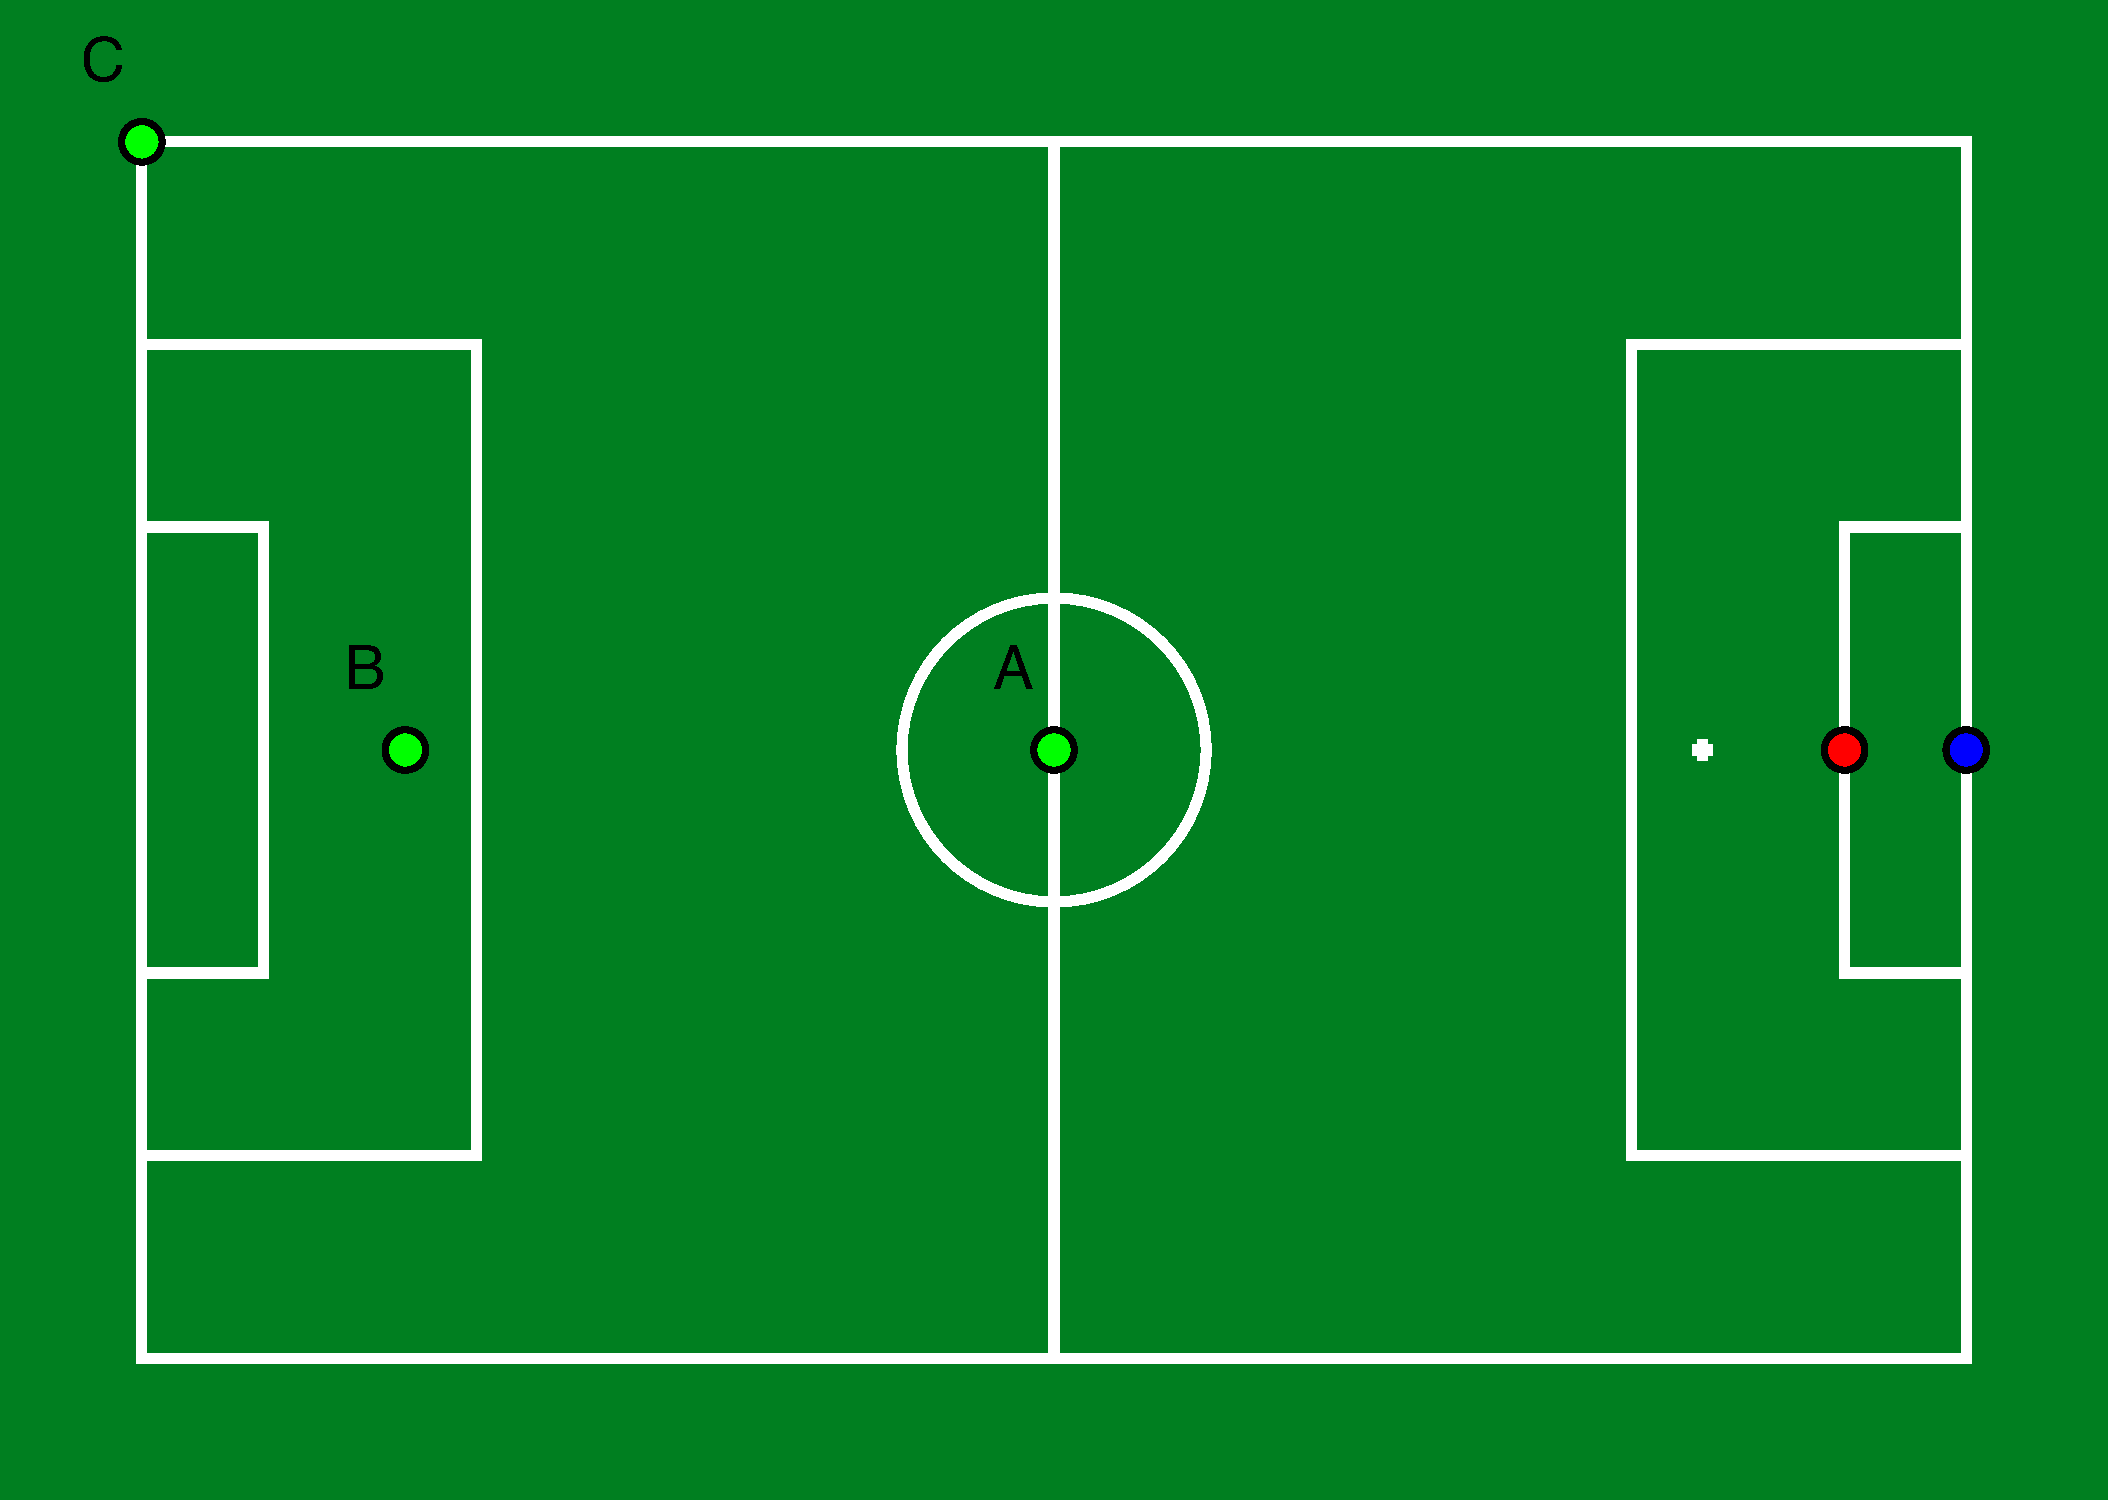
\includegraphics[width=\columnwidth]{figs/kick_leaderboard.pdf}}
    \caption{Best Kick Leaderboard: Robot completing the attempt is shown in blue, targets are shown in green, ball placement is shown in red}
    \label{fig:kick_leaderboard}
\end{figure}
\subsubsection{Challenge Execution}
Teams will be given 3 attempts at kicking to each of the 3 target postitions (illustrated in \cref{fig:kick_leaderboard}):
\begin{itemize}
    \item The centre mark in the centre circle
    \item The penalty mark on the opposite side of the field
    \item A corner on the opposite side of the field
\end{itemize}
In each attempt, participating teams must start the robot behaviour of their competing robot via a single chest button
press. The robot then has \qty{\PenaltyShootoutKickTime}{\second} to kick the ball towards the current target.
The competing robot must not touch the ball a second time after the ball has clearly moved,
otherwise the attempt ends immediately without scoring.
Once the ball has come to a complete stop, the distance from the ball to the target is measured.

Code changes are only allowed when changing targets.
\subsubsection{Scoring}
The sum of the smallest distance from each target will be recorded in the leaderboard.
Distances are rounded to the closest centimetre.

\subsection{Most Passes Leaderboard}

\subsection{Glicko Rating Leaderboard}

\subsection{Code Release}
